    \item In the circuit below, $v(t) = 3\cos \omega t$, diode cut-in voltage 0.7 V, $V_1 = 2V$, $V_2=1V$. Max and min values of $v_o(t)$ are:
    \begin{figure}[htbp]
  \centering
  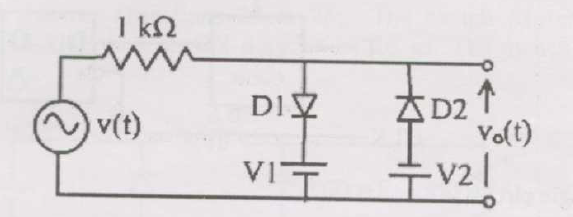
\includegraphics[width=0.6\columnwidth]{figs/2007/XE/C/fig9.png}
  \caption{Circuit}
  \label{fig:C/fig9.png}
\end{figure}
    \hfill{(2007 XE)}
    \begin{multicols}{4}
    \begin{enumerate}
        \item +2.3 V, -1.7 V
        \item +2.7 V, -1.7 V
        \item +1.3 V, -0.3 V
        \item +2.3 V, -1.3 V
    \end{enumerate}
    \end{multicols}

    \item The switch $S_1$ turns on/off repeatedly at 20 kHz, with ON duration 20 $\mu$s. Switch \& diode ideal. The average load voltage $V_o$ is:
    \begin{figure}[htbp]
  \centering
  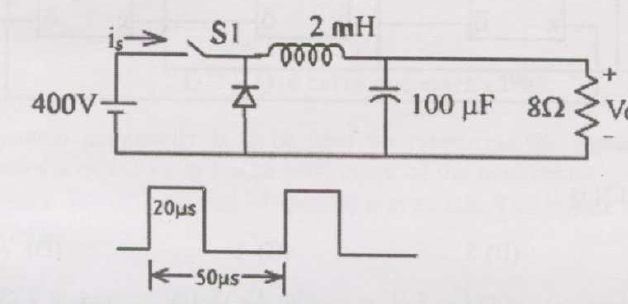
\includegraphics[width=0.6\columnwidth]{figs/2007/XE/C/fig13.png}
  \caption{Circuit}
  \label{fig:C/fig13.png}
\end{figure}
    \hfill{(2007 XE)}
    \begin{multicols}{4}
    \begin{enumerate}
        \item 667 V
        \item 400 V
        \item 240 V
        \item 160 V
    \end{enumerate}
    \end{multicols}
    

    \item Average source current $I_s$ provided by 400 V source is:
    \begin{figure}[htbp]
  \centering
  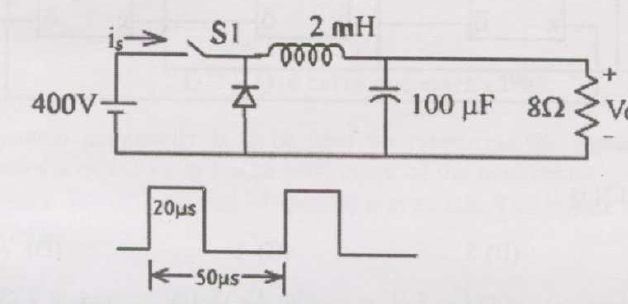
\includegraphics[width=0.6\columnwidth]{figs/2007/XE/C/fig13.png}
  \caption{Circuit}
  \label{fig:C/fig13.png}
\end{figure}
    \bigskip
    \hfill{(2007 XE)}
    \begin{multicols}{4}
    \begin{enumerate}
        \item 8 A
        \item 12 A
        \item 20 A
        \item 160 A
    \end{enumerate}
    \end{multicols}

